\documentclass{article}
\usepackage[scheme=plain]{ctex}
\usepackage{graphicx}

\title{Homework}
\author{李云浩}
\date{\today}

\begin{document}

\maketitle
\section{题目 1}
\subsection{a}
拓展顺序：Start、A、C、D、B、Goal\\
返回路径：Start $\rightarrow$ A $\rightarrow$ C $\rightarrow$ D $\rightarrow$ Goal
\subsection{b}
拓展顺序：Start、A、B、D、C、Goal\\
返回路径：Start $\rightarrow$ D $\rightarrow$ Goal
\subsection{c} 
拓展顺序：Start、A、B、D、C、Goal\\
返回路径：Start $\rightarrow$ A $\rightarrow$ C $\rightarrow$ Goal
\subsection{d}
拓展顺序：Start、A、B、C、D、Goal\\
返回路径：Start $\rightarrow$ A $\rightarrow$ B $\rightarrow$ C $\rightarrow$ D $\rightarrow$ Goal
\subsection{e}
拓展顺序：Start、A、D、B、C、Goal\\
返回路径：Start $\rightarrow$ A $\rightarrow$ C $\rightarrow$ Goal 
\section{题目 2}
(1)$g(n)$表示从初始节点到节点$n$的开销代价，$h(n)$表示从节点$n$到目标节点的估算代价。在评估函数中，
二者的系数必定大于等于0，才会与所得结果正相关。故$(2 - w ) \geq 0 \land w \geq 0 \Rightarrow 0 \leq w \leq 2$。
要保证A*算法的完备性，需要使启发式信息满足可采纳性以及一致性。\\
根据可采纳性：对于任意的节点$n$，$h(n) \leq h^*(n)$。已知当前的$h(n)$是可采纳的，即有$h(n) \leq h^*(n)$。
令$wh(n) = h'(n)$，即可将$wh(n)$整体视作一个新的启发式函数，那么为了保证可采纳性，有$h'(n) \leq h^*(n)$。
当$w \leq 1$时，有$h'(n) = wh(n) \leq h(n) \leq h^*(n)$，可以保证可采纳性。
根据一致性：对于任何的节点$n$，有$h(n) \leq cost(n, a, n') + h(n')$。由于随着与目标状态的不断接近，
$h(n') \leq h(n)$，因此$cost(n, a, n') \geq 0$。即$(2-w) \geq 0$。\\
综上所述，当$0 \leq w \leq 1$，能保证算法的最优性。\\
(2)当$w = 0$时，$f(n) = 2g(n)$。评估函数只考量了从初始节点到节点$n$的开销代价，并以此作为路径选择依据，这是一致性代价搜索算法。\\
当$w=1$时，$f(n) = g(n)+h(n)$。评估函数同时考量了初始节点到节点$n$的开销代价以及从节点$n$到目标节点的估算代价，这是A*算法。\\
当$w=2$时，$f(n)=2h(n)$。评估函数只考量了从节点$n$到目标节点的估算代价，这是只选取当前状态下的最优选择，是贪婪搜索算法。
\section{题目 3}
启发式函数：$h(n) = \lambda h_1(n) + (1 - \lambda) h_2(n)$，其中$h_1(n)$表示的是曼哈顿距离，即所有方块距离自己位置的曼哈顿距离之和。
$h_2(n)$表示的是位置错误的方块个数，$\lambda$是一个可供调节的常量，满足$0 \leq \lambda \leq 1$，来调节二者对启发式函数的影响权重。\\
因为$h_1(n)$和$h_2(n)$是可采纳的，即$h_1(n) \leq h^*(n), \quad h_2(n) \leq h^*(n)$，因此$h(n) = \lambda h_1(n) + (1 - \lambda) h_2(n) \leq h^*(n)$，故是可采纳的。\\
优劣：相比于单独的曼哈顿距离或者位置错误的方块个数，这个启发式函数综合了两者的优势，结合考虑了曼哈顿距离以及位置错误的方块个数，对局面的信息掌握得更加全面。
且该启发式函数中存在可调节因子$\lambda$，可在实际使用时不断调试，从而实现权重分配得最优化。
\section{题目 4}
\subsection{a}
\begin{figure}[h]
    \centering
    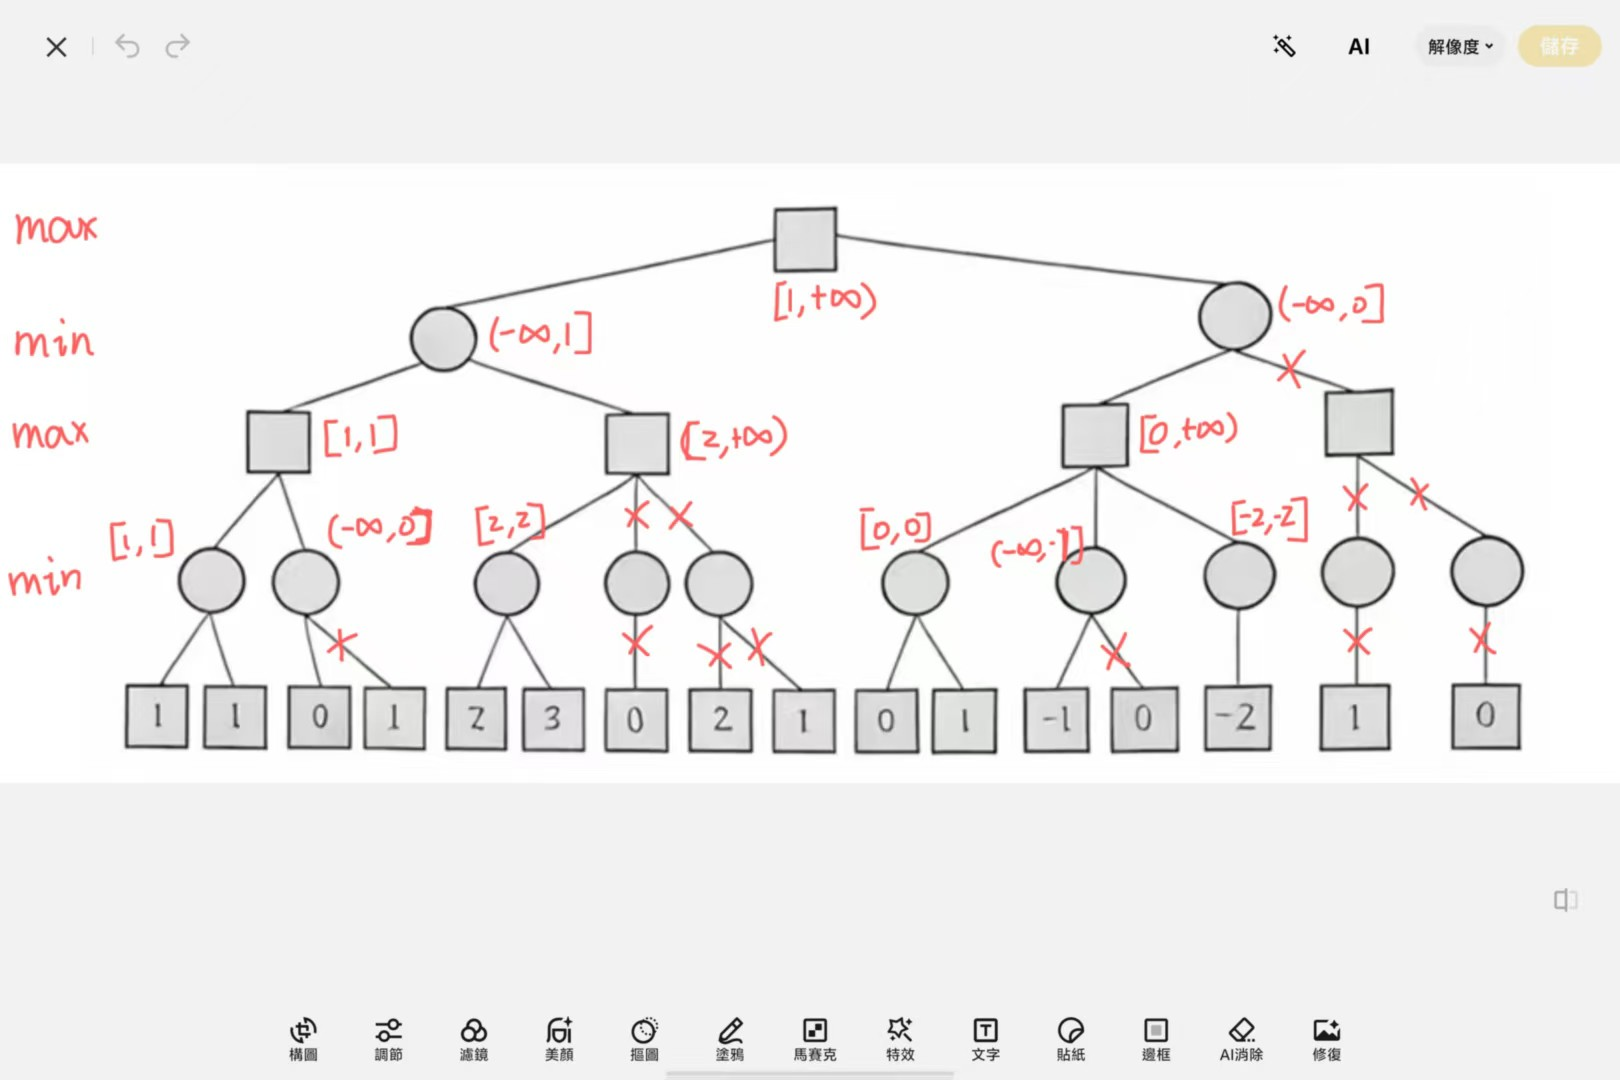
\includegraphics[width=0.75\textwidth]{T4_1.jpg}
\end{figure}
\subsection{b}
\begin{figure}[h]
    \centering
    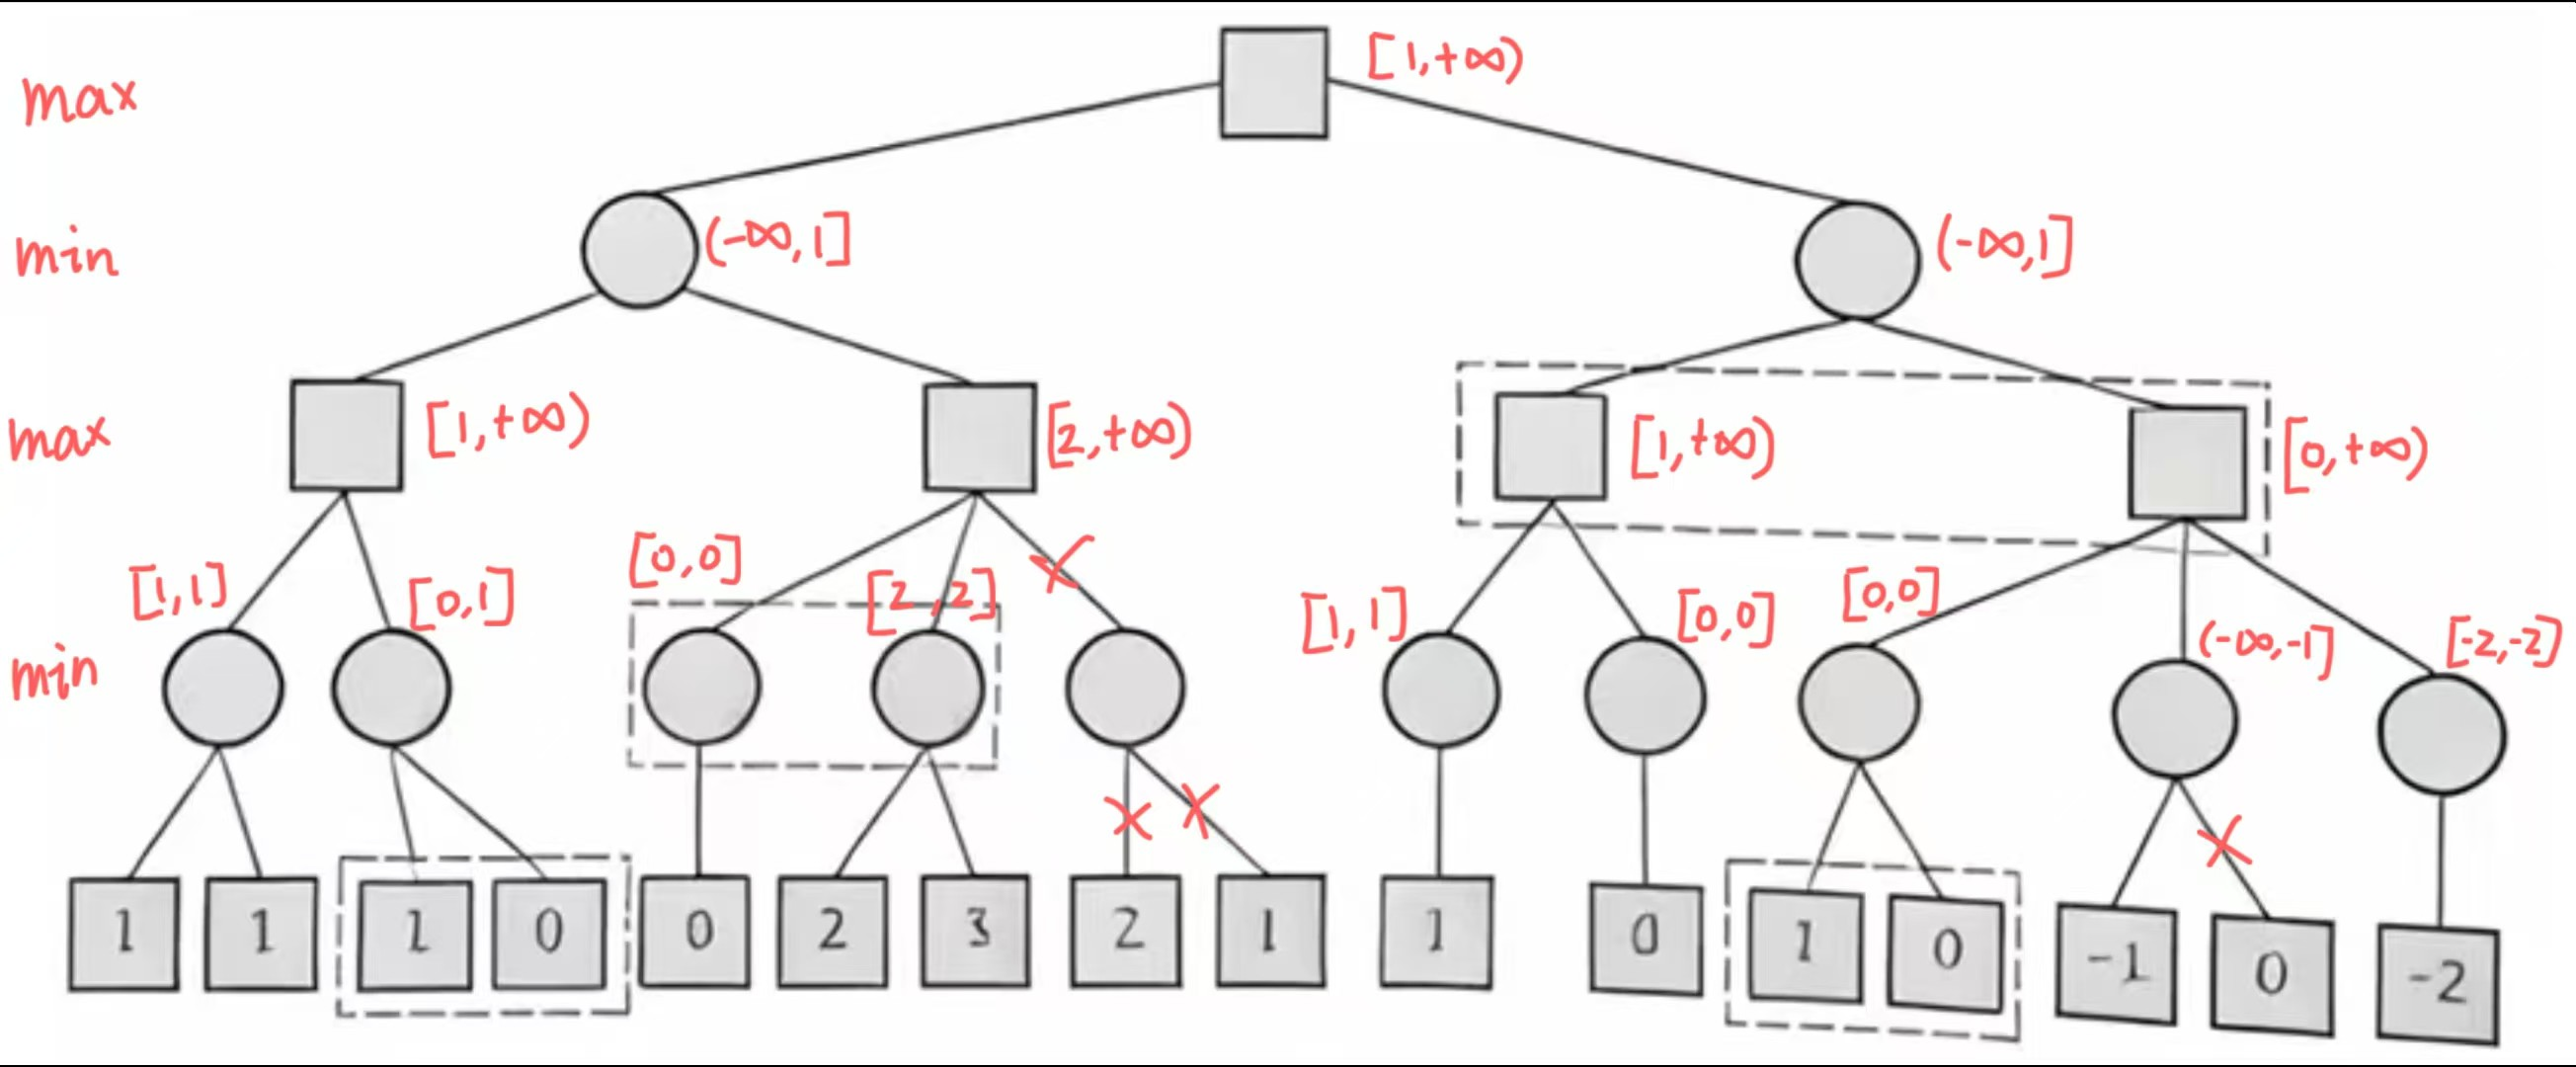
\includegraphics[width=0.75\textwidth]{T4_2.jpg}
\end{figure}
\end{document}